% Responsable: Persona 1. ~450 palabras.
\section{Fundamentos teóricos}

\subsection{Funciones analíticas y ecuaciones de Cauchy--Riemann}
% f = u + iv, u_x = v_y, u_y = -v_x. df = f'(z) dz. Contraejemplo z^2.

\subsection{Funciones armónicas y problema de Dirichlet}
% Conjugada armónica, ln|f'| = Re(ln f'), existencia y unicidad, principio del máximo.

\subsection{Esfera de Riemann y proyección estereográfica}

\subsection{Coordenada compleja sobre la esfera}
% Ejemplo de ecuación numerada:
\begin{equation}
  ds^2 = R^2\cos^2\lat\,|dw|^2, \qquad
  \sigma(w) = \frac{|f'(w)|}{R\cos\lat}
  \label{eq:sigma}
\end{equation}

% Figura 1 (Persona 3): retícula de México bajo dos proyecciones.
% \begin{figure}[ht]
%   \centering
%   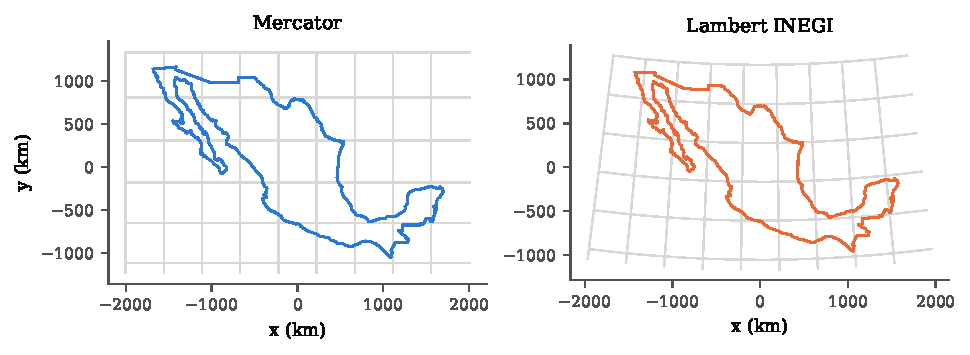
\includegraphics[width=0.9\linewidth]{fig1_reticula}
%   \caption{Retícula de meridianos y paralelos sobre México. Fuente: elaboración propia.}
%   \label{fig:reticula}
% \end{figure}
